\documentclass[tikz]{standalone}
\usepackage{xcolor, amsmath, amssymb}
\usetikzlibrary{arrows.meta}
\begin{document}

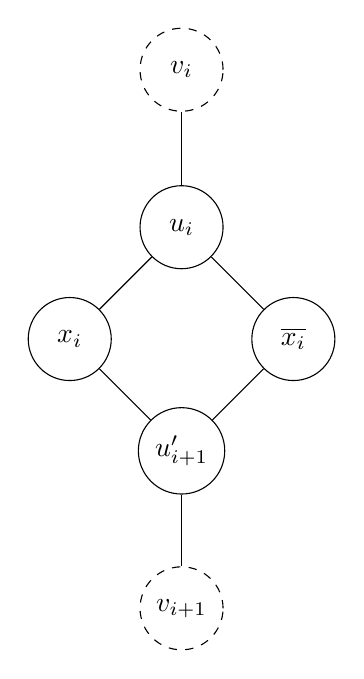
\begin{tikzpicture}[every node/.style={circle,draw},scale=2,minimum size=30pt]
\node[dashed] at(0,1.71)(v){$v_i$};
\node at(0,0.71)(u){$u_i$};
\node at(0,-0.71)(u'){$u_{i+1}'$};
\node[dashed] at(0,-1.71)(v'){$v_{i+1}$};
\node at(-0.71,0)(x){$x_i$};
\node at(0.71,0)(x'){$\overline{x_i}$};
\path(u)edge(v)edge(x)edge(x')
     (u')edge(v')edge(x)edge(x');
\end{tikzpicture}

\end{document}